\RequirePackage{docswitch}
\setjournal{\flag}


\documentclass[]{emulateapj}

\usepackage{lsstdesc_macros}

\usepackage{xspace}
\usepackage{graphicx}
\graphicspath{{./}{./figures/}{.logos}}
\bibliographystyle{apj}


\newcommand{\textul}{\underline}
\newcommand{\qp}{\texttt{qp}}
\newcommand{\pz}{photo-$z$ PDF}
\newcommand{\Pz}{Photo-$z$ PDF}
\newcommand{\mgdata}{bright\xspace}
\newcommand{\Mgdata}{Bright\xspace}
\newcommand{\ssdata}{faint\xspace}
\newcommand{\Ssdata}{Faint\xspace}


\begin{document}

\title{ Approximating photo-z PDFs for large surveys }


\begin{abstract}

Upcoming and ongoing galaxy surveys will produce redshift probability 
distribution functions (PDFs) in addition to traditional photometric redshift 
(photo-$z$) point estimates.
However, the storage of \pz s may present a challenge with increasingly large 
catalogs, as we face a trade-off between the accuracy of subsequent science 
measurements and the storage cost.
This paper presents \qp, a Python package facilitating manipulation of 
approximations of 1-dimensional PDFs, as suitable for \pz s.
We use \qp\ to investigate the performance of three simple PDF storage formats 
on two realistic mock datasets, representative of upcoming surveys with 
different data qualities, as a function of the number of stored parameters per 
\pz, using metrics of both individual \pz s and an estimator of the overall 
redshift distribution function.

\end{abstract}

\dockeys{methods: data analysis, catalogs, surveys}

\maketitlepost





\section{Introduction}
\label{sec:intro}


Ongoing and upcoming wide-field imaging surveys such as the Large Synoptic 
Survey Telescope 
(LSST)\footnote{\url{https://www.lsst.org/}}\citep{ivezic_lsst:_2008} will 
observe billions of galaxies; studies of cosmology and galaxy evolution with 
these data will rely on the method of photometric redshift (photo-$z$) 
estimation.
Photo-$z$s are subject to a number of systematic errors, some caused by the 
estimation procedures and others intrinsic to the data itself.
The photo-$z$ community has come to favor methods that provide a redshift 
probability distribution function (PDF) that includes information about the 
potential for such systematic errors for each galaxy in the survey.

Given the tremendous size of the surveys in question, storage of these 
probability distributions involves making difficult decisions.
Each survey seeks to create a catalog of \pz s balancing accuracy against 
storage cost.
For example, the \pz\ catalog that LSST will release will be limited to 
$\sim100$ floating point numbers per galaxy\citet[section 
4.2.2]{juric_data_2017}, with plans to store \pz s derived by multiple methods.
The problem of \pz\ approximation for large surveys was first addressed in 
\citet{carrasco_kind_sparse_2014} in the context of a single galaxy survey, a 
limited set of \pz\ approximation schemes, and metrics appropriate for 
deterministic, not probabilistic, objects.
However, we expect the choice of \pz\ approximation, and the number of stored 
parameters associated with it, will depend on the science case and its 
requirements on \pz\ accuracy: different science cases will need different 
accuracy metrics.
In this paper, we address the question of \textit{how} these choices should be 
made in general, by providing the publicly available \qp\ Python 
package\footnote{\url{https://github.com/aimalz/qp}} to enable each survey to 
optimize their \pz\ approximation via mathematically motivated and 
science-driven metrics.
We demonstrate this approach on two sets of realistic mock data.

In Section~\ref{sec:methods}, we outline how \qp\ can be used to optimize the 
choice of \pz\ parametrization.
In Section~\ref{sec:data}, we describe the mock datasets on which we perform 
such an analysis.
We present the results of this procedure in Section~\ref{sec:results} and make 
recommendations for the use of \qp\ by the photo-$z$ community in 
Section~\ref{sec:conclusions}.








\section{Methods}
\label{sec:methods}



We have developed the \qp\ Python package to facilitate the parametrization and 
approximation of \pz s.
A \texttt{qp.PDF} object can carry a number of different parametrizations, each 
associated with a representation.
Conversions between parametrizations are facilitated by the 
\texttt{numpy}\footnote{\url{http://www.numpy.org/}}, \texttt{scipy} 
\footnote{\url{https://www.scipy.org/}}, and 
\texttt{scikit-learn}\footnote{\url{http://scikit-learn.org}} 
\citep{pedregosa_scikit-learn:_2011} tools.
The currently supported parametrizations are described in 
Section~\ref{sec:approx}.
The \qp\ package also provides a few built-in metrics of the accuracy of a 
representation of a \pz\ relative to a given parametrization that has been 
designated as the reference representation.
Built-in plots are made using 
\texttt{matplotlib}\footnote{\url{https://matplotlib.org/}}.
The currently implemented metrics are described in Section~\ref{sec:metric}.
Large-scale tests can be conducted using the \texttt{qp.Ensemble} class that 
provides a wrapper for parallelized operations over collections of 
\texttt{qp.PDF} objects; parallelization is facilitated by the \texttt{pathos} 
\footnote{\url{http://trac.mystic.cacr.caltech.edu/project/pathos/wiki.html}} 
\citep{mckerns_building_2012, mckerns_pathos:_2010} package.

\subsection{Approximation Methods}
\label{sec:approx}

First, we establish a vocabulary for the definitions of approximation methods.
Each \textit{parametrization} of a \pz\ is defined in terms of the 
\textit{format} function $\mathcal{F}$, \textit{metaparameters} $\vec{C}$, and 
\textit{parameters} $\vec{c}$.
A parametrization in turn corresponds to a \textit{representation}
\begin{align}
  \label{eq:definition}
  \hat{p}^{\mathcal{F}, \vec{C}, \vec{c}}(z) &\equiv \mathcal{F}_{\vec{C}}(z; 
\vec{c})
\end{align}
of the \pz, denoted as $\hat{p}(z)$ for brevity.
We often employ interpolation schemes with a generic interpolator function 
$F_{\vec{C}'}(z; \vec{c})$ that comes with its own metaparameters $\vec{C}'$.
\qp\ supports all interpolation options available to the 
\texttt{scipy.interpolate.interp1d} function, but we choose a default 
interpolation scheme for each format to maximize the fidelity of the 
approximations to the original, high-resolution PDFs.

\qp\ supports conversion of \pz\ approximations between five formats: step 
functions, samples, quantiles, evaluations, and mixture model components.
These formats may be associated with any number $N_{f}$ of stored parameters 
$c_{i}$ per \pz%, which are presumed to be floating point numbers unless 
otherwise specified.
Meanwhile, the metaparameters $C_{i}$ are the set of numbers necessary to 
convert the stored \pz\ parameters $\vec{c}$ into a PDF over redshift.
In this work we consider special cases of three of these formats as candidates 
for large survey \pz\ catalog storage: regular binning 
(Section~\ref{sec:bins}), random samples (Section~\ref{sec:samples}), and 
regular quantiles (Section~\ref{sec:quantiles}), while the other two, 
evaluations and mixture models, are used solely for internal manipulations 
within \qp.

We have not yet included the 
\texttt{SparsePz}\footnote{\url{https://github.com/mgckind/SparsePz}} sparse 
basis representation of \citet{carrasco_kind_sparse_2014}, which uses a mixture 
model of $N_{f}$ members of a library of $\sim10^{4}$ functions and has 
impressive compression properties.
We omit this format because decomposition with \texttt{SparsePZ} does not 
enforce that the stored parametrization be a probability distribution in the 
mathematical sense of nonnegativity and integration to unity.
While normalizing the integral of a positive semidefinite function is always 
possible (if the endpoints of integration are specified), one can motivate 
multiple schemes for enforcing nonnegativity that result in different 
reconstructions $\hat{p}(z)$.
We postpone to future work the exploration of adaptations of non-positive 
semidefinite representations and inclusion of the sparse basis representation 
in \qp, restricting ourselves to mixture models of 
\texttt{scipy.stats.rv\_continuous} objects.

The various \qp\ formats are illustrated in Figure~\ref{fig:qp} on a multimodal 
\pz\ with stored parameters.
\begin{figure}
  \begin{center}
    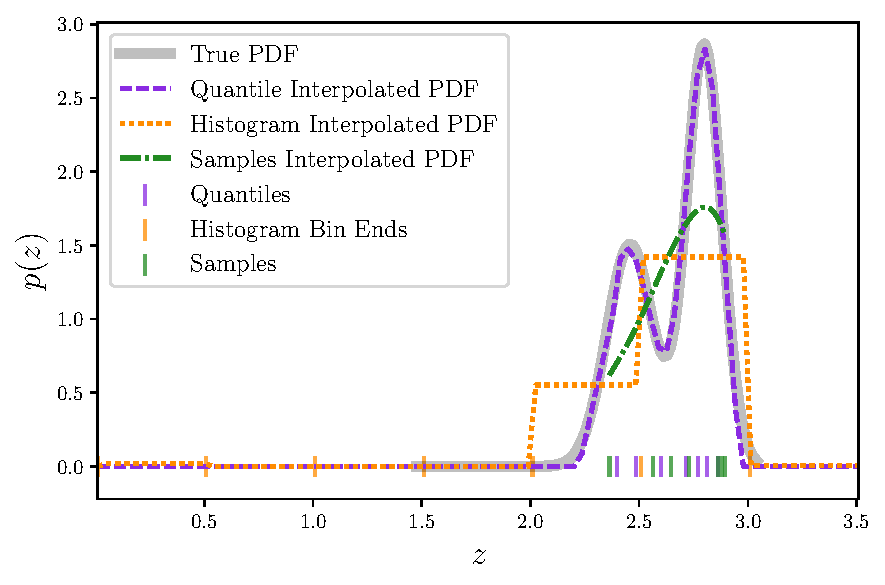
\includegraphics[width=\columnwidth]{figures/demo_pz.pdf}
    \caption{\qp\ approximation of a continuous 1-dimensional PDF (solid black 
line) using the step function (orange dotted line), samples (green dash-dotted 
line), and quantile formats (purple dashed line) with the same number of stored 
parameters ($N_{f}=7$ in this case).
    \label{fig:qp}}
  \end{center}
\end{figure}

For each format, we address the following questions:
\begin{itemize}
  \item When/where has this format appeared in the literature as a published 
catalog format, native \pz\ code output format, and science application input 
format?
  \item What exactly is stored under this format, per galaxy (the parameters) 
and per catalog (the metaparameters)?
  \item Beyond fidelity to the original \pz, what are the a priori strengths 
and weaknesses of this format?
\end{itemize}

\subsubsection{Regular Binning}
\label{sec:bins}

By far the most popular format for approximating and storing \pz s is that of a 
piecewise constant step function, also called a histogram binning 
\citep{carrasco_kind_somz:_2014, sadeh_annz2:_2016, cavuoti_metaphor:_2017}.
It is the only format that has been used for public release of \pz\ catalogs 
\citep{tanaka_photometric_2017, sheldon_photometric_2012}; it is unclear 
whether this is a consequence or cause of the fact that it is the most common 
format for using \pz s in cosmological inference, as tomographic binning is a 
universal step between the \pz\ catalog and calculation of any two-point 
correlation function.

The metaparameters of the binned parametrization are the ordered list of 
redshifts $\vec{C} = (z_{1}, z_{2}, \dots, z_{N_{f}}, z_{N_{f}+1})$ serving as 
bin endpoints shared by all galaxies in the catalog, each adjacent pair of 
which is associated with a parameter $c_{i}=\int_{C_{i}}^{C_{i+1}}\ p(z)dz$.
The \qp\ histogram format assumes $p(z)=0$ when $z<C_{1}$ or $z>C_{N_{f}+1}$, 
leading to the normalization condition $\sum_{i} c_{i}(C_{i+1}-C_{i})) = 1$.
\footnote{Note that this is not generally equivalent to the erroneous 
normalization condition $\sum_{i} c_{i} = 1$ commonly enforced in public 
catalogs.}
The histogram format function $\mathcal{F}^{h}$ is the sum of a set of $N_{f}$ 
step functions, making the reconstructed estimator of the \pz
\begin{align}
  \label{eq:binned}
  \hat{p}^{h}(z) &= \sum_{i}^{N_{f}}\ c_{i} 
\left\{\begin{tabular}{cc}$1$&$C_{i}<z<C_{i+1}$\\
0&$z < C_{i}$\ or\ $z > C_{i+1}$\end{tabular}\right\},
\end{align}
where the step functions may be considered their own interpolators.
Here we only consider a regular binning, with $C_{i+1}=C_{i}+\delta_{f}$ for a 
constant $\delta_{f}=(C_{N_{f}+1}-C_{1})/N_{f}$, as this is the only type of 
binning that has been used in the literature, but this condition is not 
required by \qp.

The regular histogram format may be considered wasteful in terms of data 
storage; a \pz\ with a very compact (broad) probability distribution may have 
many parameters taking the same value $c_{i}\approx0$ 
($c_{i}\approx(C_{N_{f}+1}-C_{1})\delta^{-1}$) that are redundant in storage.

\subsubsection{Random Samples}
\label{sec:samples}

Samples are the native output format of many machine learning algorithms due to 
the discrete nature of training sets \citep{de_vicente_dnf_2016}.
Such approaches typically produce large numbers of samples, far more than can 
realistically be stored by any survey, so a subsample is commonly stored.
Samples are easy to use in standard science applications developed for redshift 
point estimates, so they have an established presence in the literature.

The parameters of the samples format are the $N_{f}$ samples $\vec{c}=(z_{1}, 
z_{2}, \dots, z_{N_{f}-1}, z_{N_{f}})$, where $C=N_{f}$ is an implicit 
metaparameter.
Though it is possible to construct a catalog where $C$ is not uniform over the 
catalog, but is instead somehow optimized for each galaxy, we leave its 
investigation to future work, as it has not yet appeared in the literature.
The format function $\mathcal{F}^{s}$ that turns samples into a representation 
of the \pz\ is simply the interpolator $F$; in the tests presented here, we use 
the Gaussian kernel density estimate (KDE) of 
\texttt{scipy.stats.gaussian\_kde} with the smoothing bandwidth $C'$ as a 
metaparameter.  The samples representation is then
\begin{align}
  \label{eq:sampled}
  \hat{p}^{s}(z) &= F_{C'}(z; \vec{c}).
\end{align}

Though samples are an obvious choice for \pz s with narrow features of high 
amplitude, we expect that using a small number of samples from a broad \pz\ may 
increase the variance of any ensemble metrics, as the sampling introduces 
additional shot noise.
The researcher must also choose an interpolation method to reconstruct a \pz\ 
from samples.

\subsubsection{Regular Quantiles}
\label{sec:quantiles}

One parametrization that has not previously been investigated in the context of 
photometric redshifts is that of quantiles, which are defined in terms of the 
cumulative distribution function (CDF).
The quantile format for expressing a PDF, however, has appeared in the 
astronomy literature \citep{sun_star_2015, pizzocaro_results_2016, 
laycock_x-ray_2017}.

Under the quantile format, a \pz\ catalog shares $N_{f}$ ordered CDFs 
$\vec{C}=(q_{1}, q_{2}, \dots, q_{N_{f}-1}, q_{N_{f}})$.
Each galaxy's catalog entry is the vector of redshifts $\vec{c}=(z_{1}, z_{2}, 
\dots, z_{N_{f}-1}, z_{N_{f}})$ satisfying $CDF(c_{i})=C_{i}$, so the quantile 
format function $\mathcal{F}_{q}$ is the derivative of an interpolation of the 
inverse CDF $CDF^{-1}(C_{i})=c_{i}$ under the interpolation scheme $F$.
In this study, we test regular quantiles $C_{i}\equiv i(N_{f}+1)^{-1}$ using a 
\texttt{scipy.interpolate} spline interpolation scheme in the quantile range 
and linear extrapolation outside it.
The format function is then the convolution $\mathcal{F}^{q}=F(CDF^{-1})$, 
making the quantile representation
\begin{align}
  \label{eq:quantiles}
  \hat{p}^{q}(z) &= F\left(z; \vec{c}, 
\frac{\Delta\vec{C}}{\Delta\vec{c}}\right).
\end{align}


A quantiles parametrization (the namesake of the \texttt{qp} code) is expected 
to be an efficient approximation for \pz s because it allocates storage evenly 
in the space of probability density.
In contrast, the histogram format stores data evenly spaced in redshift, and 
the samples format stores data randomly in probability density.
As with the samples representation, an interpolation function must be chosen 
for reconstructing the \pz\ from the stored parameters.
Depending on the native \pz\ output format, converting to the quantile format 
may require $N_{f}$ numerical optimizations to find the quantiles.
We accelerate these optimizations by initializing at rough, approximate 
quantiles based on CDF evaluations on a grid.





\subsection{Comparison Metrics}
\label{sec:metric}

In this work, our aim is to probe how closely \pz s reconstructed from limited 
set of stored parameters approximate their original, high-resolution 
representation.
This is done without reference to a galaxy's true redshift; there is, in fact, 
no notion of a true redshift in our analysis.
(For a demonstration of how one might approach the distinct problem of 
evaluating the accuracy of a \pz\ relative to a true redshift, see Schmidt, et 
al.\ in preparation.)
The loss of information, measured in nats (base $e$ bits), incurred when using 
an approximation of the PDF $\hat{P}(z)$ instead of the best possible 
representation of the  PDF $P(z)$ is given by the Kullback-Leibler divergence 
(KLD), which is defined as
\begin{align}
  \label{eq:kld}
  \mathrm{KLD}[P(z) || \hat{P}(z)] &= \int_{-\infty}^{\infty}\ P(z)\ 
\log\left[\frac{P(z)}{\hat{P}(z)}\right]\ dz,
\end{align}
where $\log$ is the natural logarithm throughout this paper.

The most important feature of the KLD is its asymmetry; it is not a distance, 
like the root mean square error, that is the same from $P(z)$ to $P'(z)$ as it 
is from $P'(z)$ to $P(z)$ but a \textit{divergence} in the information lost 
when using $P'(z)$ to approximate $P(z)$.
The KLD requires that both functions $P(z)$ and $P'(z)$ be probability 
distributions (always positive semidefinite and integrating to unity); this may 
need to be explicitly enforced for some approximation formats.
The KLD is always positive, and a smaller value indicates better agreement 
between the approximation and the truth.
We review the properties of the KLD and provide some intuition for it in the 
Appendix.

Because there is in general no closed-form expression for the KLD, we calculate 
the discrete KLD
\begin{align}
  \label{eq:kld_approx}
  \mathrm{KLD}[P(z) || \hat{P}(z)] &\approx 
\delta_{ff}\sum_{z=z_{1}}^{z_{N_{ff}}}\ P(z)\ 
\log\left[\frac{P(z)}{\hat{P}(z)}\right]
\end{align}
using evaluations of the PDF under each format on a very fine, regular grid 
$(z_{1}, z_{2}, \dots, z_{N_{ff}-1}, z_{N_{ff}})$ with resolution 
$\delta_{ff}\ll\delta_{f}$.

\subsubsection{Individual \pz s}
\label{sec:individual_metric}

Some science applications rely on the recovery of individual galaxy \pz s that, 
for example, may be used as the basis for targeting spectroscopic follow up for 
a variety of science applications.
For this purpose, we calculate the KLD of each individual \pz\ in our catalogs 
and then characterize the distribution of KLD values (which is itself a PDF) by 
its first, second, and third moments (the mean, variance, and kurtosis, 
respectively).
We use these aggregate statistics to observe how the approximate individual \pz 
s for each dataset vary with the choice of parametrization.

\subsubsection{Stacked $\hat{n}(z)$ estimator}
\label{sec:stacked_metric}

In cosmology, \pz s have thus far been used almost exclusively to estimate the 
redshift distribution function $n(z)$ necessary for calculating the correlation 
functions used by many cosmological probes.
The most common way to estimate the redshift distribution function for a sample 
of $N_{g}$ galaxies is to sum the \pz s according to
\begin{align}
  \label{eq:nz}
  \hat{n}(z) &\equiv \frac{1}{N_{g}}\ \sum_{k=1}^{N_{g}}\ \hat{p}_{k}(z).
\end{align}
Here, the estimator is normalized so that it, too, is a PDF.
While we do not recommend this approach to estimating the redshift distribution 
(see Malz and Hogg, et al.\ (in preparation)), we use it here on the assumption 
that any metric calculated on a more principled estimator will have similar 
behavior with respect to the parametrization of the \pz\ catalog.
Our primary metric is therefore the KLD \textit{from} the stacked estimator of 
a catalog of evaluations of reconstructed \pz s \textit{to} the stacked 
estimator of a catalog of evaluations of the original, high-resolution \pz s.


\section{Photo-z Test Data}
\label{sec:data}

With the expectation that the optimal parametrization for approximating \pz s 
may differ according to the properties of the original photometric data, we 
demonstrate a procedure for vetting \pz\ parametrizations on a pair of mock 
datasets, each intended to be realistic projections of the anticipated LSST \pz 
s.
All \pz s were fit using the publicly available Bayesian Photometric Redshift 
(BPZ) code \citep{benitez_bayesian_2000}, which employs spectral energy 
distribution (SED) fitting to a template library.
The choice of \pz\ estimation method, however, is not relevant to this study; 
so long as the mock \pz s are \textit{realistically complex}, meaning they take 
shapes similar to those we expect to see in \pz s from real datasets with 
similar photometric properties, it does not matter whether the \pz s produced 
by BPZ are accurate redshift posteriors.
We seek only to optimize the fidelity of the stored \pz\ relative to the \pz\ 
output by a representative \pz\ fitting code.
\citep[See][Schmidt, et al.\ in preparation for other work comparing the 
accuracy of \pz s produced by different methods.]{tanaka_photometric_2017}
Because we believe that each galaxy has an underlying redshift interim 
posterior probability distribution that is a continuous function, to which the 
output of BPZ is itself a high-resolution approximation in the form of 
evaluations on a grid, we fit the gridded \pz\ with a Gaussian mixture model 
that we designate as the reference representation for our accuracy tests.

\subsection{\Mgdata data mock catalog}
\label{sec:graham}

Our first dataset is an $N_{g}=100,000$ object subset of the simulated galaxy 
catalog used for LSST photometric redshift experiments by 
\citet{graham_photometric_2017}.
The data builds on the Millennium simulation \citep{springel_simulations_2005}, 
and in particular the LC DEEP catalog based on the galaxy formation models of 
\citet{gonzalez-perez_how_2014}, and was created using the lightcone 
construction techniques described by \citet{merson_lightcone_2013}.
We limit the sample to galaxies with a catalog $i$-band magnitude of $i<25$ and 
true redshifts $z<3.5$.
As in Graham, et al. (in preparation), we simulate observed apparent magnitudes 
from the true catalog magnitudes by adding a normal random scatter with a 
standard deviation equal to the predicted magnitude error for each galaxy (from 
Section 3.2.1. of \citet{ivezic_lsst:_2008}, using the software of 
\citet{connolly_end--end_2014}, assuming a mean airmass of 1.2 and a 10-year 
accumulation of 56, 80, 184, 184, 160, and 160 visits in filters $ugrizy$, 
respectively).
We also ignore any magnitudes fainter than the predicted 10-year limiting 
magnitudes in each filter, $u<26.1$, $g<27.4$, $r<27.5$, $z<26.1$, and 
$y<24.9$, as a realistic simulation of non-detections.

The \pz\ estimates for this simulated catalog use the CFHTLS set of spectra 
\citep{ilbert_accurate_2006} as BPZ templates and the default parameter 
settings for BPZ, except that we impose a maximum photometric redshift of 3.5 
and allow BPZ to use the $i$-band as a magnitude prior during the photo-$z$ fit.
The \pz s from BPZ are in the form of $N_{ff} = 351$ evaluations of the 
probability density on a regular grid of redshifts $0.01 < z < 3.51$, a 
subsample of which are plotted in Figure~\ref{fig:graham_pzs}.

\begin{figure}
  \begin{center}
    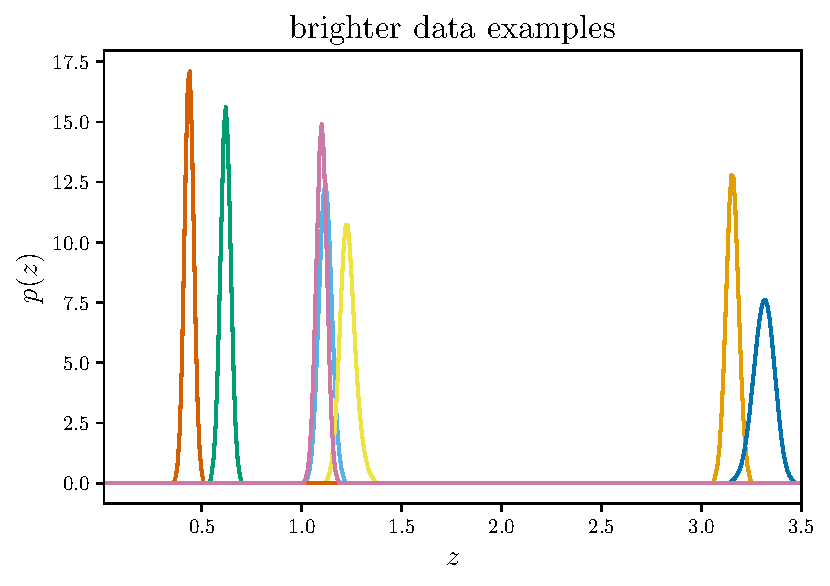
\includegraphics[width=\columnwidth]{figures/graham_pzs.pdf}
    \caption{Example \pz s from the mock LSST data of Graham, et al.\ (in 
preparation).
    The \mgdata mock photometry yields largely narrow, unimodal \pz s.
    \label{fig:graham_pzs}}
  \end{center}
\end{figure}

As the figure shows, the \pz s from this dataset tend to be unimodal and 
sharply peaked, as if coming from brighter photometric data due to the 
conservative cuts in photometric magnitudes of this dataset.
We produce reference \pz s for the analysis by fitting a three-component 
Gaussian mixture model to each \pz\ in the catalog.
We then calculate the three approximations to each \pz\ and evaluate their 
accuracy using the metrics described above.

\subsection{\Ssdata mock catalog}
\label{sec:schmidt}

Our second dataset is an independent simulation of the expected LSST galaxy 
sample.
Here, we use the Buzzard-highres-v1.0 mock galaxy catalog of deRose, et al.\ 
(in preparation) of galaxies with SEDs drawn from an empirical library of 
$\sim500,000$ SEDs from the Sloan Digital Sky Survey (SDSS).
Given an SED, redshift, and absolute $r$-band magnitude for each galaxy, we 
compute the expected apparent magnitudes and magnitude errors in the six 
broadband LSST filters ($ugrizy$), assuming the full 10-year depth of the 
survey using the simple model of \citet{ivezic_lsst:_2008}.
The catalog contains $N_{g}\approx100,000$ galaxies $z<2.105$ to a depth of 
$i<26.9$, 1.5 magnitudes deeper than the expected LSST Gold sample of galaxies 
that will have $S/N\gtrsim30$ in multiple bands.

In implementing BPZ, we createed a custom Bayesian prior using a subset of the 
Buzzard-highres-v1.0 catalog and a spanning template set via a simple k-means 
clustering algorithm based on $100$ of the SDSS SEDs used in creating the 
Buzzard catalog.
BPZ produces \pz s in the format of probability density evaluations on a 
regular grid of $N_{ff}=211$ redshifts $0.005\leq z\leq2.105$, a subsample of 
which are plotted in Figure~\ref{fig:schmidt_pzs}.

\begin{figure}
  \begin{center}
    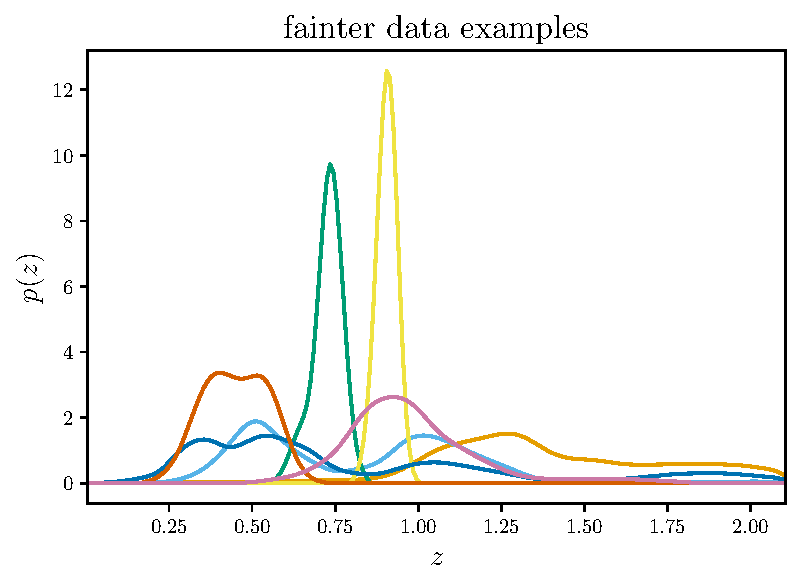
\includegraphics[width=\columnwidth]{figures/schmidt_pzs.pdf}
    \caption{Example \pz s from the mock LSST data of deRose, et al.\ (in 
preparation).
    This sample contains a higher proportion of broad and/or multimodal \pz s, 
as if from the \ssdata data.
    \label{fig:schmidt_pzs}}
  \end{center}
\end{figure}

Even with six filters spanning the optical, there are known degeneracies 
(e.~g.~the Lyman/Balmer break degeneracy) that lead us to expect the presence 
of multimodal \pz s.
The exceptional depth of the dataset also leads us to expect the presence of 
broad \pz s.
We produced reference \pz s for the analysis by fitting a five-component 
Gaussian mixture model to each gridded \pz\ in the catalog.
We then calculated the three different approximations to each \pz, and 
evaluated their accuracy using the metrics described above.


\section{Results \& Discussion}
\label{sec:results}



We calculate the metrics of Section~\ref{sec:metric} on 10 random 
instantiations of catalogs of $N_{g}=100$ galaxies drawn randomly from each of 
the datasets discussed in Section~\ref{sec:data} and with each of $N_{f}=3,\ 
10,\ 30,\ 100$ stored parameters.
We then illustrate how our results could be used to choose an appropriate 
parametrization for each dataset given constraints on the distribution of KLDs 
of individual \pz s, the KLD for $\hat{n}(z)$, or $N_{f}$


\subsection{Stacked $\hat{n}(z)$ estimator}
\label{sec:stacked_results}

Figure~\ref{fig:stacked} shows an example of $\hat{n}(z)$ estimated from \pz s 
reconstructed from just $N_{f}=10$ parameters under each of our three 
approximation formats, evaluated on the same fine grid as the input \pz s.
The strong features in the curve are due to the very small sample size of $100$ 
galaxies.
As expected, the stacked histogram is quite coarse because of the step function 
interpolation.
The samples and quantiles can be interpolated such that the stacked $n(z)$ 
estimator of the approximation is almost indistinguishable from the stacked 
estimator of the original, high-resolution \pz s.


\begin{figure}
  \begin{center}
    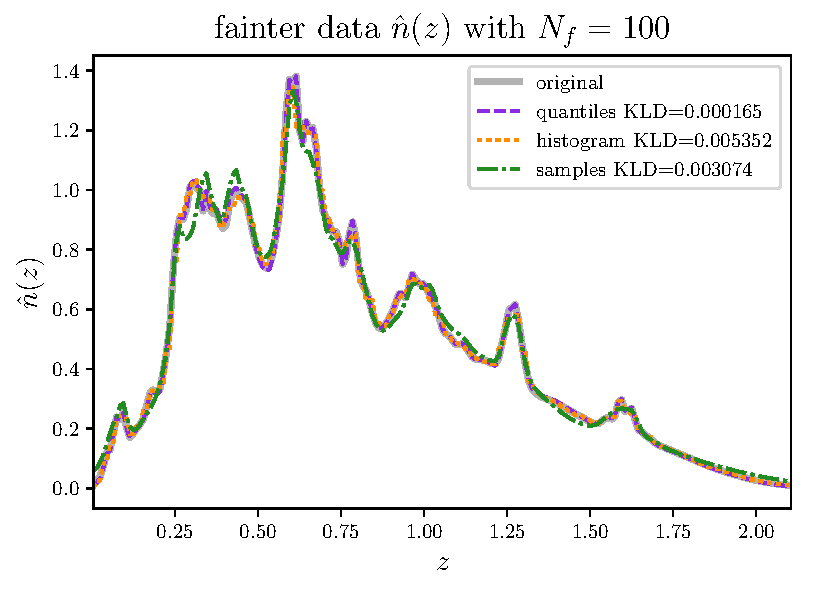
\includegraphics[width=\columnwidth]{figures/stacked.pdf}
    \caption{An example of the stacked estimator of the redshift distribution, 
for a subsample of $N_{g}=100$ galaxies drawn from the \ssdata data mock 
catalog and with just $N_{f}=10$ parameters used for each \pz; the small-scale 
features are due to the small number of galaxies in the sample.
    The most striking characteristic of $\hat{n}(z)$ with a relatively small 
number of parameters on a small number of galaxies is the coarseness of the 
histogram format (orange dotted line) relative to the quantile format (purple 
dashed line) and samples format (green dash-dotted line), both of which are 
fairly close to $\hat{n}(z)$ derived from evaluating the original, 
high-resolution \pz s (thick gray line).
    \label{fig:stacked}}
  \end{center}
\end{figure}

The $\hat{n}(z)$ KLD values for each parametrization on both mock datasets are 
collected and plotted in Figure~\ref{fig:kld}, with error regions based on the 
variance between the 10 instantiations.
The two datasets share some features:
\begin{enumerate}
\item The histogram format leads to substantial loss of information relative to 
the other formats.
\item The samples and quantile formats have similar KLDs, particularly at low 
$N_{f}$.
\item The quantile format achieves the lowest KLD of all formats in the high 
$N_{f}$ regime.
\item The samples format is more consistent in terms of the variance between 
instantiations.
\item The samples format asymptotically approaches a limit in KLD at 
$N_{f}\geq30$, likely because that is the limit at which the samples-induced 
shot noise becomes subdominant.
\end{enumerate}
Because the data quality has a significant impact on the behavior of the 
metric, we proceed to discuss the two datasets separately, in terms of relative 
performance between formats and absolute $\hat{n}(z)$ KLDs as a function of 
$N_{f}$.


For the \mgdata data mock catalog, the histogram format not only has a 
consistently higher $\hat{n}(z)$ KLD but one that does not improve with 
increasing $N_{f}$.
This poor performance independent of resource allocation is actually expected 
because, due to the narrow, unimodal \pz s of Figure~\ref{fig:graham_pzs}, a 
great majority of the probability density will fall into a single bin $c^{\ 
h}_{i=j}$ with all other $c^{\ h}_{i\neq j}\approx 0$ \textit{regardless} of 
$N_{f}$.
The quantile format consistently produces the lowest $\hat{n}(z)$ KLDs, with a 
larger improvement over the samples format as $N_{f}$ increases.
The improvement with larger $N_{f}$ is a surprising result because the shot 
noise due to samples should decrease with higher $N_{f}$.
The quantile format also has a larger variance between instantiations than the 
samples format, likely due to the imperfections of the procedures for deriving 
the quantile parameters $\vec{c}^{\ q}$ from the original, high-resolution 
$p(z)$ and for reconstructing $\hat{p}^{q}(z)$ from the quantile parameters 
$\vec{c}^{\ q}$.

In the \ssdata data mock catalog, the histogram format does improve with 
increasing $N_{f}$, however, it takes a whopping $N_{f}=100$ stored parameters 
before the histogram format can supercede the KLD of the samples and quantile 
formats at a mere $N_{f}=3$ stored parameters, where the histogram format takes 
a staggering value $KLD>1$.
With \pz s that take nontrivial values across a wider range of redshifts, the 
histogram format is expected to capture more structure with more bins, 
consistent with the aforementioned improvement.
The samples format's asymptote is surprisingly achieved at a lower KLD for the 
\ssdata data mock catalog than for the \mgdata data mock catalog.
The variance between instantiations of the quantile format increases at high 
$N_{f}$, a possible indication of room for improvement with the procedures for 
deriving the quantile parameters $\vec{c}^{\ q}$ from the original, 
high-resolution $p(z)$ and for reconstructing $\hat{p}^{q}(z)$ from the 
quantile parameters $\vec{c}^{\ q}$

\begin{figure*}
  \begin{center}
    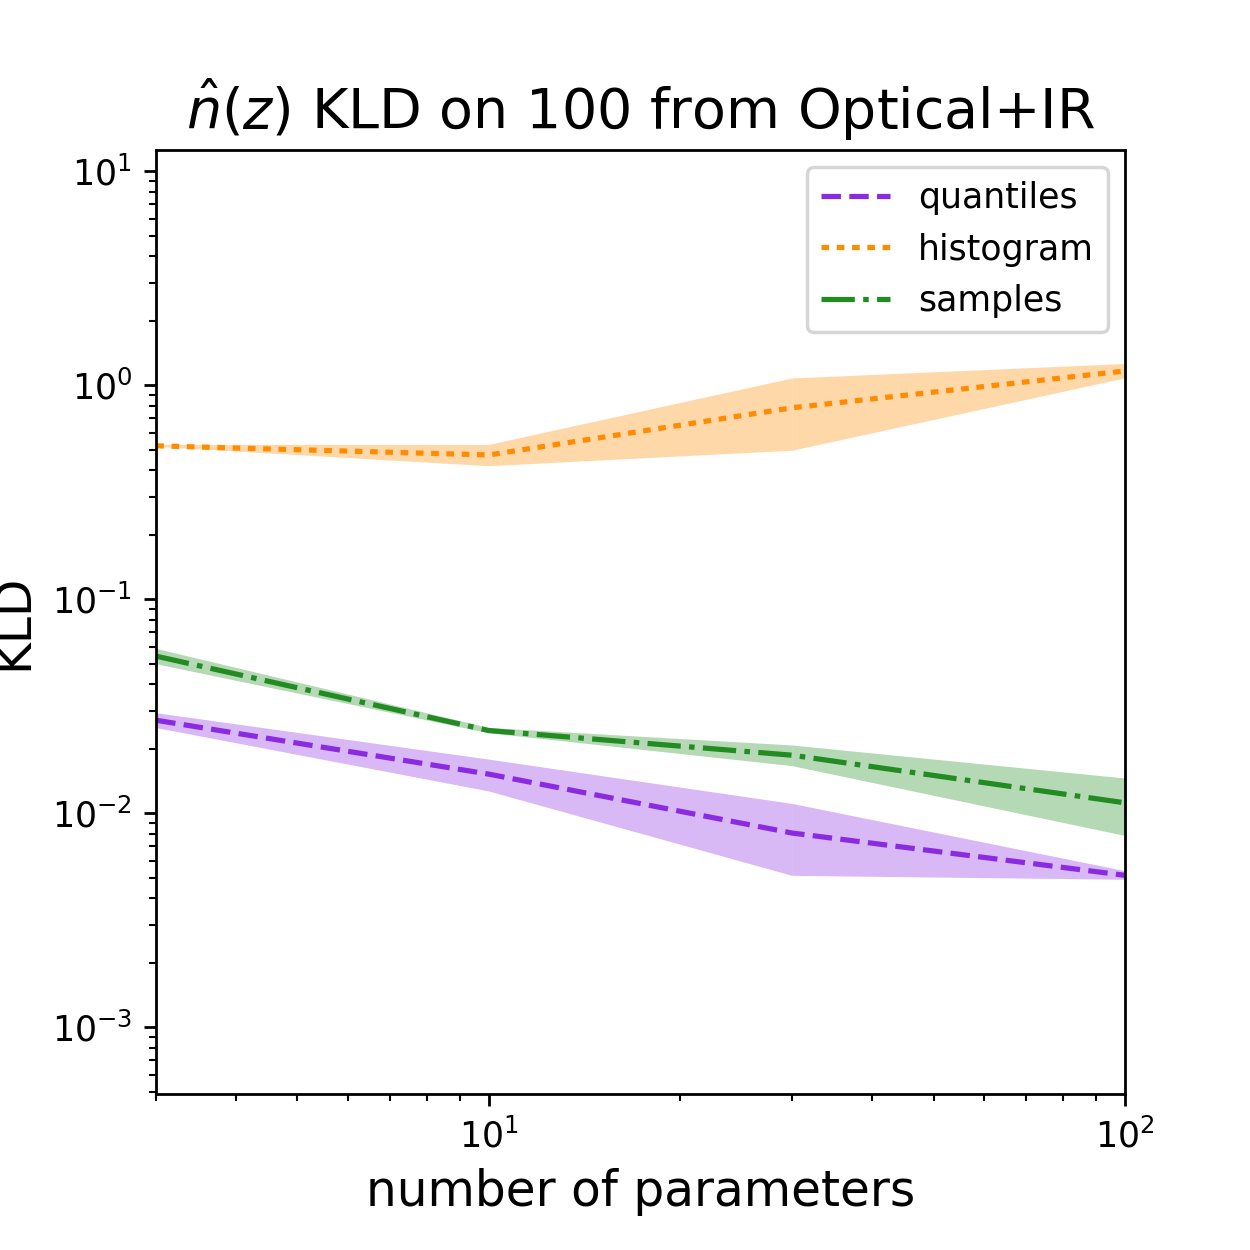
\includegraphics[width=\columnwidth]{figures/graham_kld.png}    
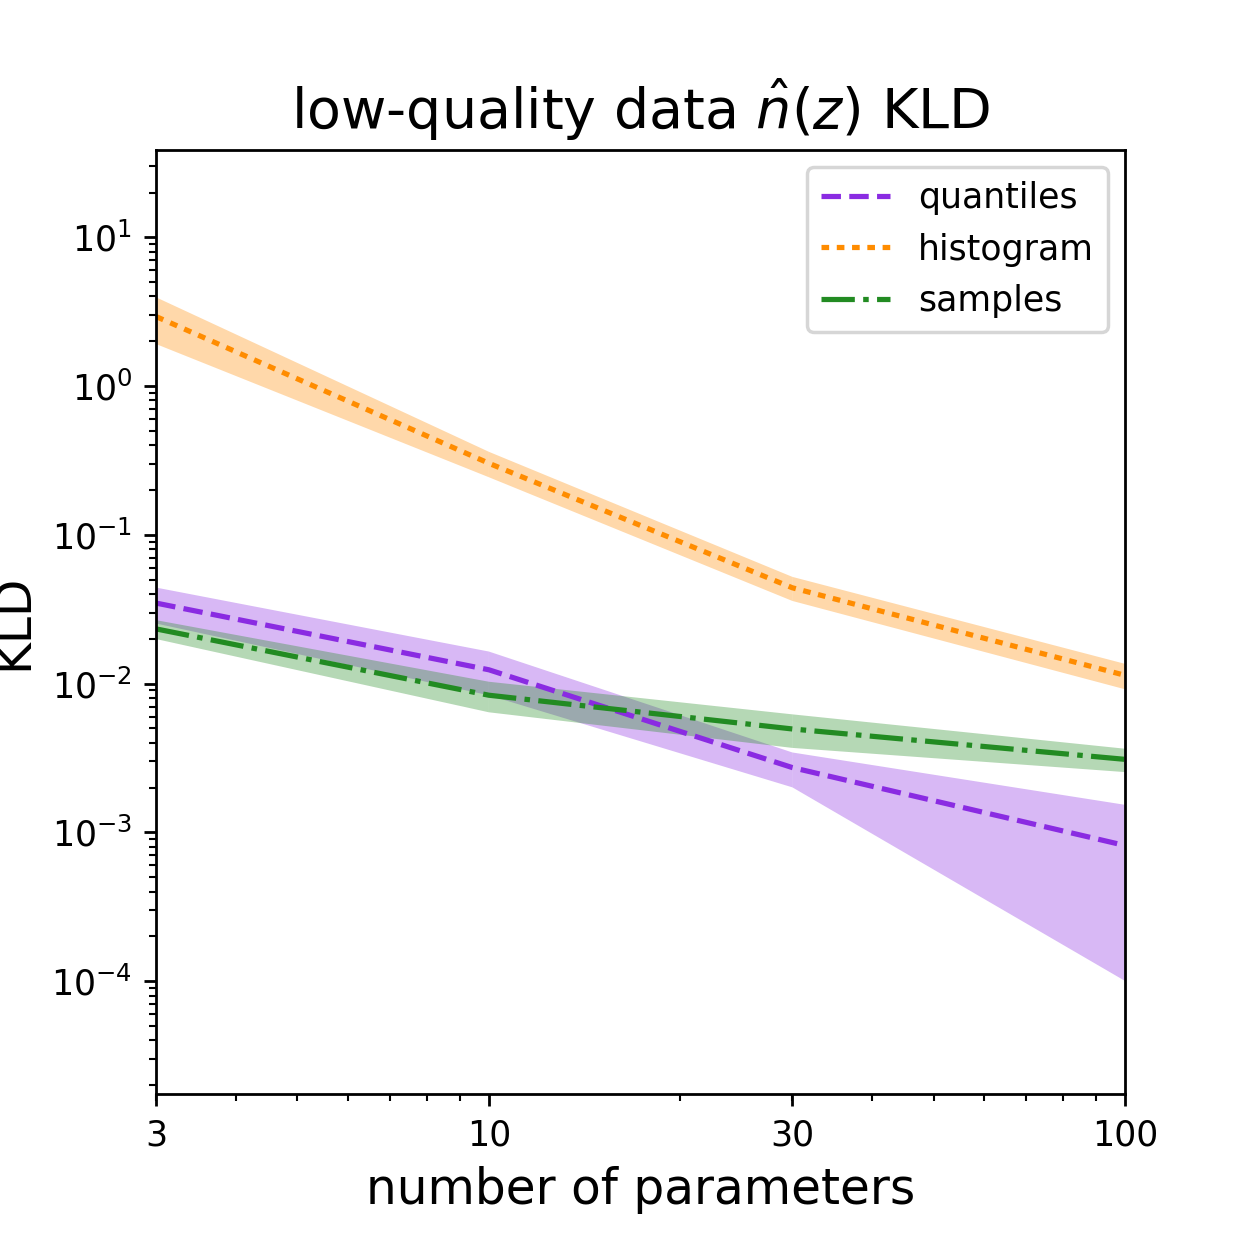
\includegraphics[width=\columnwidth]{figures/schmidt_kld.png}
    \caption{KLD between $\hat{n}(z)$ derived from approximate pz\ 
representations and  $\hat{n}(z)$ derived from the original, high-resolution 
\pz s as a function of number of stored parameters, for the three different 
approximation schemes: quantiles (purple dashed line), samples (green 
dash-dotted line), and histogram (orange dotted line).
    Left panel: The mock catalog of \mgdata data of Section~\ref{sec:graham} 
favors the quantiles format and strongly disfavors the histogram format, with 
quantiles being slightly more favorable than samples.
    Right panel: The histogram format is not well-suited to the mock catalog of 
\ssdata data of Section~\ref{sec:schmidt}, while the quantiles and samples 
formats perform comparably well.
    \label{fig:kld}}
  \end{center}
\end{figure*}

We interpret Figure~\ref{fig:kld} in the context of constraints on storage 
allocation imposed by the survey and constraints on the acceptable degree of 
information loss imposed by the science requirements.
The former corresponds to a vertical line at a given $N_{f, lim}$ in Fig. 
\ref{fig:kld}; the best format would be the one that achieves the lowest KLD at 
$N_{f, lim}$.
The latter corresponds to a horizontal line at $KLD_{lim}$ in 
Figure~\ref{fig:kld}; the best format would be the one that achieves 
$KLD_{lim}$ at the smallest value of $N_{f}$.
If there is some flexibility in the acceptable degree of information loss on 
$\hat{n}(z)$ and/or the allocation of storage for \pz s, as is the case for 
LSST, it may be best to examine the asymptotic behavior of the KLD as a 
function of $N_{f}$ for each format considered.
For example, if the KLD can be significantly reduced with a slightly larger 
$N_{f}$, it may be possible to request additional storage capacity for the 
survey's \pz s.


\subsection{Individual \pz s}
\label{sec:individual_results}

We also compare our three parametrizations on the basis of the distributions of 
the KLD calculated for every \pz\ in the dataset's ensemble.
An example of the individual \pz\ KLD distribution is shown in 
Figure~\ref{fig:individual} with $N_{f}=10$.

\begin{figure}
  \begin{center}
    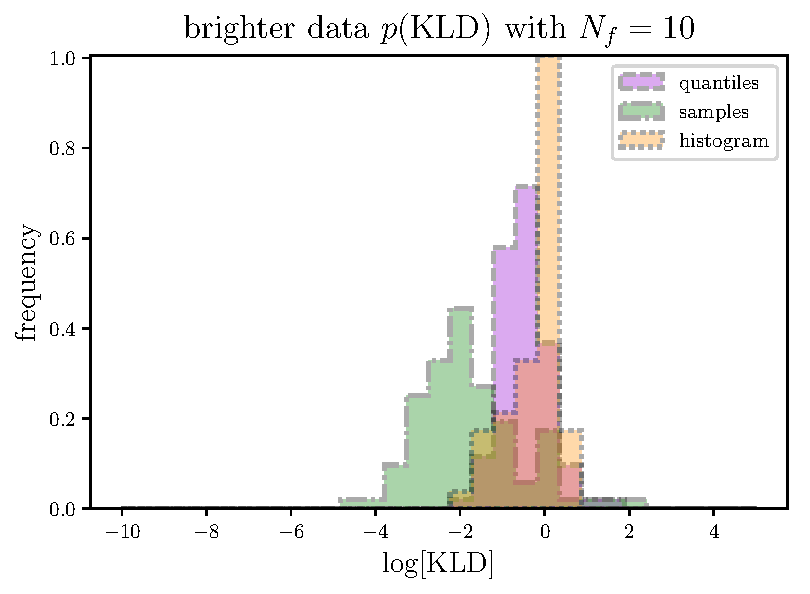
\includegraphics[width=\columnwidth]{figures/individual_kld.pdf}
    \caption{The distribution of log-KLD values for $N_{g}=100$ \pz s from the 
\mgdata dataset with $N_{f}=10$ over the quantiles (purple with dashed border), 
samples (green with dash-dotted border), and histogram (orange with dotted 
border) formats.
    For the individual \pz s, the piecewise constant format has a higher median 
KLD than the samples or quantile formats, which are comparable to one another.
    \label{fig:individual}}
  \end{center}
\end{figure}

To distill what is observed in plots like Figure~\ref{fig:individual} for both 
datasets and all parametrizations, we compare the moments of the distributions 
of metric values for the distribution of the KLDs of individual \pz s under 
each parametrization, summarized in Figure~\ref{fig:moments}.
While it is obvious that one would like the mean (first moment) of the KLD 
distribution to be low, interpretation of higher-order moments is less clear.
In a science application that is robust to \pz\ outliers, a parametrization 
with a high variance (second moment) may be acceptable, whereas in another 
science application that simply requires well-characterized errors could 
tolerate a higher mean in exchange for a lower variance.
To meaningfully interpret the KLDs of individual \pz s, it will be necessary 
for those using \pz s in their science to calculate the requirements on the 
acceptable degree of information loss.

\begin{figure*}
  \begin{center}
    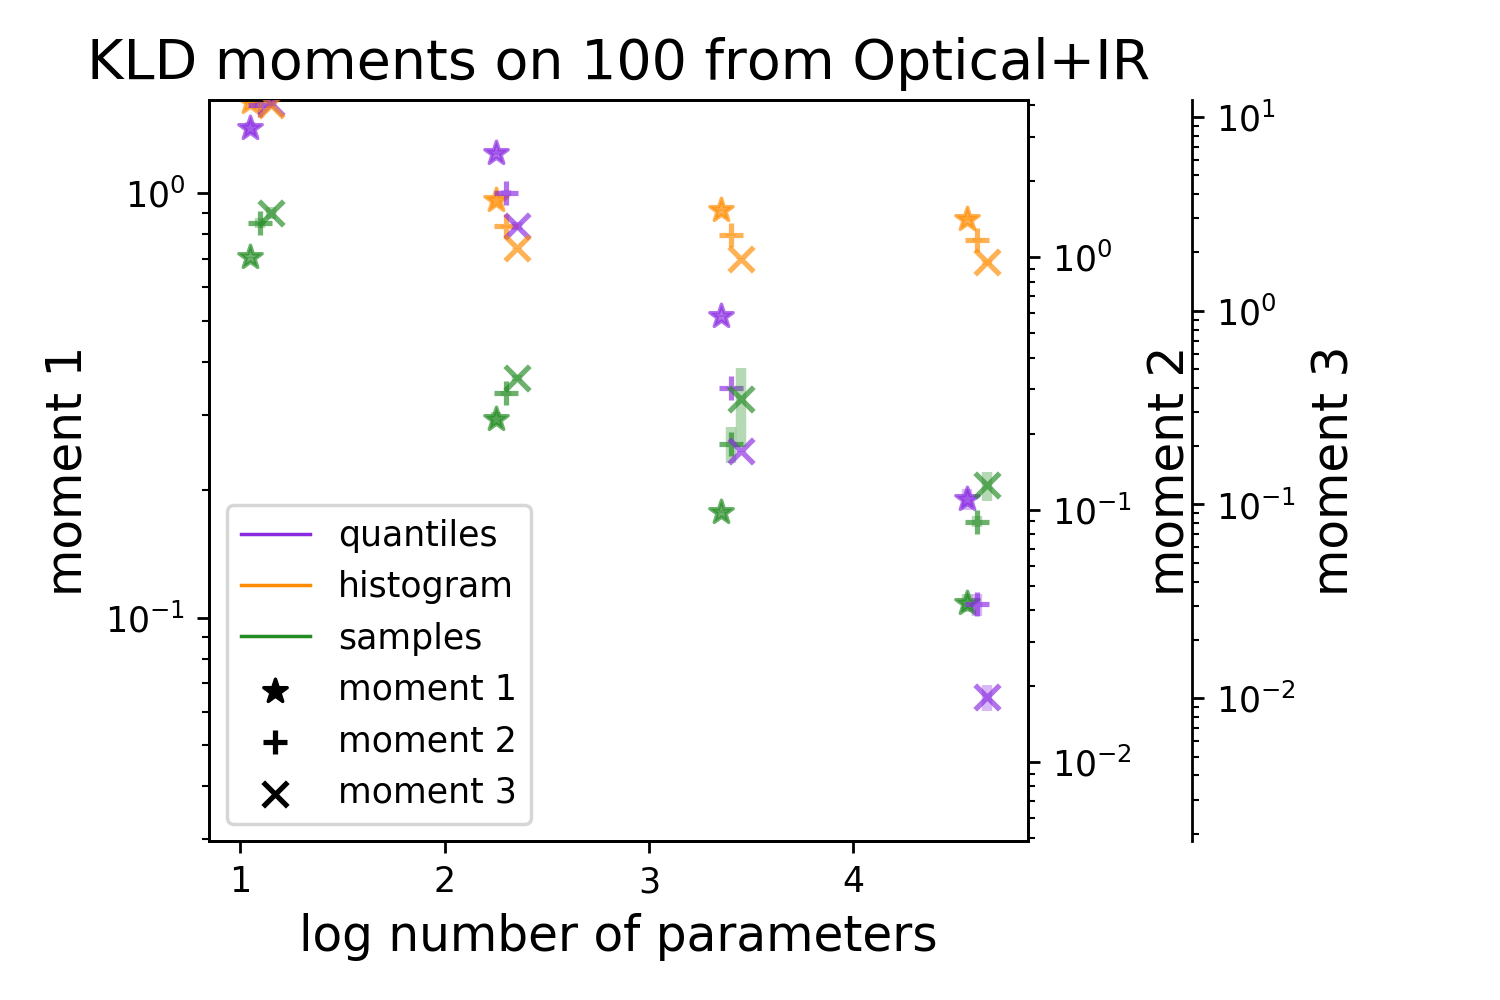
\includegraphics[width=\columnwidth]{graham_moments.png}    
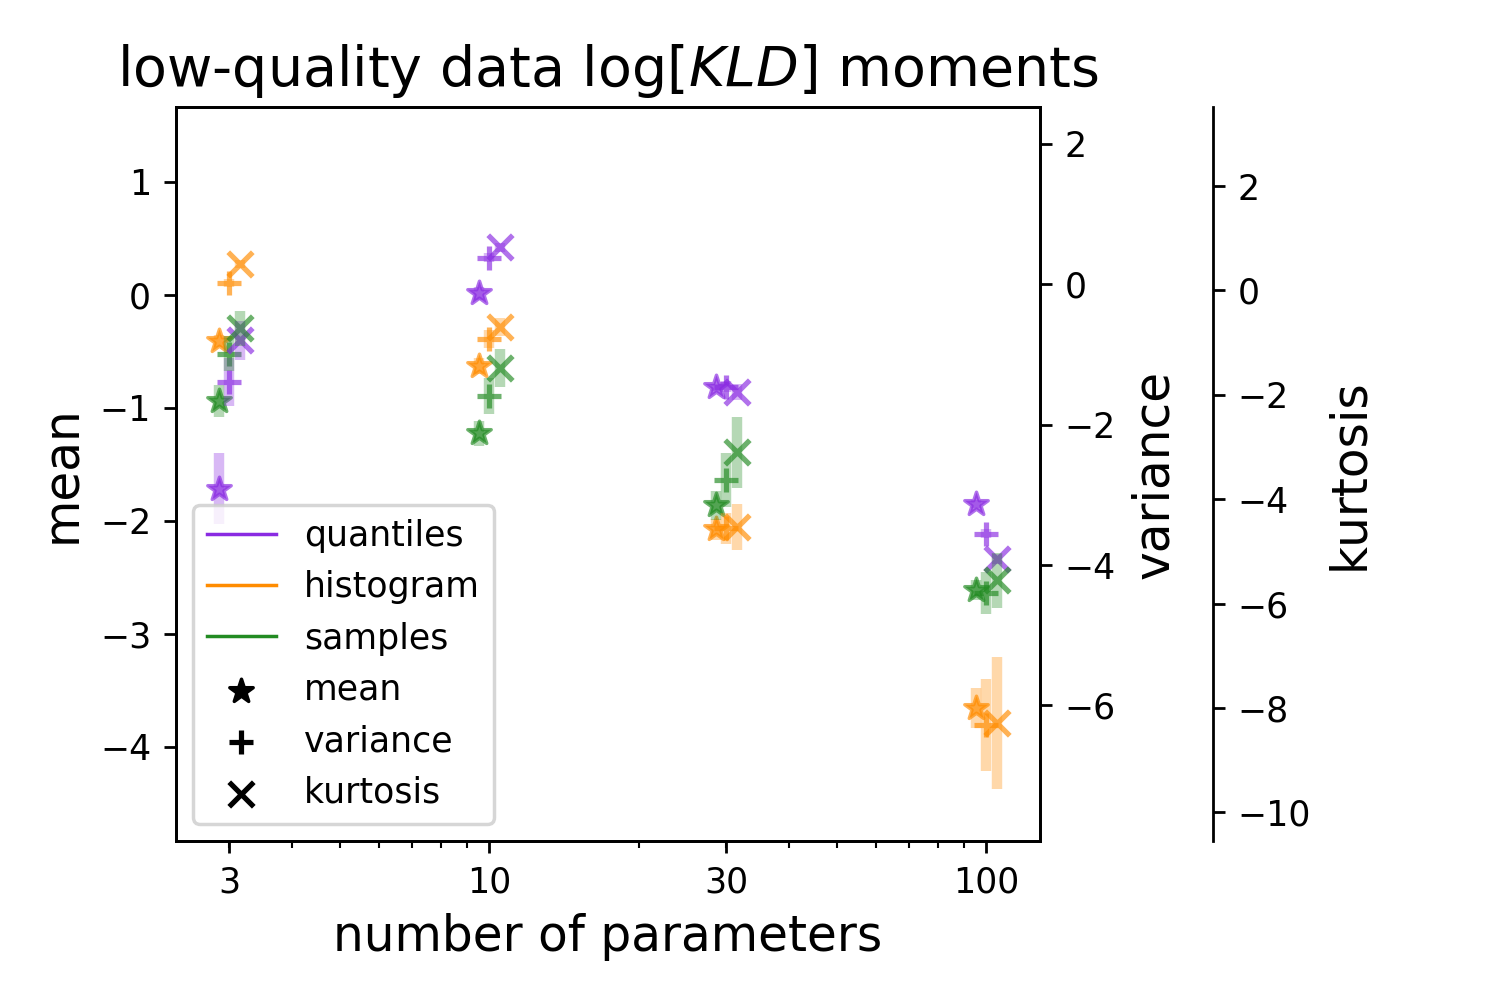
\includegraphics[width=\columnwidth]{schmidt_moments.png}
    \caption{The mean ($\bigstar$), variance ($+$), and kurtosis ($\times$) of 
the log-KLD distributions for each dataset as a function of $N_{f}$ for the 
quantile (purple), samples (green), and histogram (orange) formats.
    The moments and their error regions are offset about $N_{f}$ to improve 
readability.
    Left panel: The samples format consistently minimizes the moments of the 
log-KLD distribution of the \mgdata data mock catalog at low $N_{f}$, and the 
moments are similar across formats at the highest $N_{f}=100$.
    Right panel: The\ssdata data mock catalog exhibits no clear pattern at low 
$N_{f}$ but the moments of all formats decrease at high $N_{f}$ with the 
histogram format achieving the lowest moments in that regime.
    \label{fig:moments}}
  \end{center}
\end{figure*}






\section{Conclusions \& Future Directions}
\label{sec:conclusions}


This work develops a principled approach to choosing a parametrization for 
storing a catalog of \pz s from a survey of known data quality to balance the 
accuracy of \pz s and science products thereof reconstructed from the stored 
parameters against the available storage constraints.
We demonstrate the recommended method on two realistic mock datasets 
representative of upcoming \pz\ catalogs and draw the following conclusions:
\begin{itemize}
  \item The optimal parametrization depends on the properties of the data and 
the science-driven metric used.
  \item A larger number of available parameters in which to store a \pz\ 
catalog does not necessarily imply a significant reduction in loss of 
information.
  \item The histogram format has a high rate of loss of information over 
brighter and fainter data mock catalogs and across a wide range of number of 
stored parameters, particularly under an aggregate function of individual 
reconstructed \pz\ approximations.
  \item The samples format is an excellent option for storage of brighter \pz\ 
catalogs, balancing loss of information for both individual \pz\ s and a 
catalog-wide metric.
  \item The quantile format is a promising option for minimizing loss of 
information in \pz\ storage, competitive with samples for an estimator of the 
redshift distribution function.
\end{itemize}

Given the constraint that LSST will be able to store only 200 floating point 
numbers to quantify the redshift of each galaxy and intends to include the 
results of several \pz\ codes, we can safely say that LSST can store the output 
of more than one \pz\ code without risk of significant loss of information.
We do not advocate for a one-size-fits-all solution to the problem and 
emphasize that the optimal choice must depend on the requirements of the 
science metric(s) and characteristics of the underlying \pz\ catalog.

Though we discussed the previous use of each format in science calculations, we 
do not endorse the preference of any format on the basis of existing 
infrastructure for its use.
Rather, we hope that the community will continue to develop analysis methods 
that best make use of the information in \pz s and then choose parametrizations 
that most effectively serve the needs of those intended practices.

We invite the community to contribute additional formats and metrics to the 
publicly available \qp\ Python package developed for this project.  \qp\ is a 
tool that can be used to optimize the choice of stored parametrization of a 
catalog of \pz s based on the accuracy needs of the use cases of the catalog.


\subsection*{Appendix}
\label{sec:kld}

We develop some intuition for the Kullback-Leibler Divergence by contrasting it 
with the familiar metric of the root-mean-square error (RMSE)
\begin{align}
  \label{eq:rmse}
  \mathrm{RMSE} &= \sqrt{\int (P(z) - \hat{P}(z))^{2} dz}.
\end{align}
Consider the simple example of a Gaussian $P(z)=\mathcal{N}(\mu_{0}, 
\sigma_{0}^{2})$ being approximated by a Gaussian $P'(z)=\mathcal{N}(\mu, 
\sigma^{2})$, whose KLD is
\begin{align}
  \label{eq:gaussian}
  \mathrm{KLD} &= 
\frac{1}{2}\left(\log\left[\frac{\sigma^{2}}{\sigma_{0}^{2}}\right] + 
\frac{\sigma_{0}^{2}}{\sigma^{2}} + \frac{(\mu-\mu_{0})^{2}}{\sigma^{2}} - 
1\right)
\end{align}
To get a sense of the units of information, we can calculate the KLD and RMSE 
in some limiting cases.
If $\sigma=\sigma_{0}$ but $\mu=\mu_{0}+1$, we obtain 
$\mathrm{KLD}=\frac{1}{2}$ nat -- if the mean of the approximation is wrong by 
an additive factor of $1\sigma$, half a nat of information is lost.
If $\mu=\mu_{0}$ but $\sigma=\sqrt{2\pi}\sigma_{0}$, we find 
$\mathrm{KLD}\approx\frac{1}{2}$ nat -- half a nat of information is also lost 
if the variance of the approximation is off by a multiplicative factor of 
$2\pi$.

We can use the KLD to identify notions of imprecision and inaccuracy.
Intuitively, precision must be related to how close $\sigma$ is to $\sigma_{0}$ 
and accuracy must be related to how close $\mu$ is to $\mu_{0}$.

If $\mu\approx\mu_{0}$, we can say $\mathrm{KLD}\sim\log[r] + \frac{1}{2}r^{-2} 
- \frac{1}{2}$ where $r^{-1}\equiv\frac{\sigma_{0}}{\sigma}$ is a measure of 
\textit{precision}, whose behavior is illustrated in 
Figure~\ref{fig:precision}, alongside that of the RMSE.  We observe that an 
overestimated variance increases the KLD as the log of the square root of the 
ratio of the estimated variance to the true variance.

\begin{figure}
  \begin{center}
    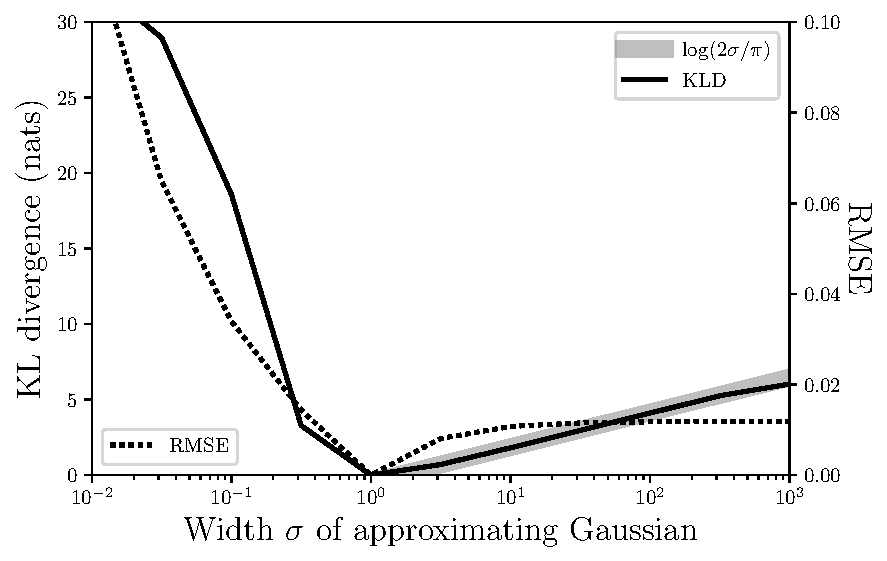
\includegraphics[width=\columnwidth]{figures/precision.pdf}
    \caption{The KLD (solid black line) is proportional to the log of the 
inverse precision $r$ for $\sigma>\sigma_{0}$, behavior that is qualitatively 
similar to that of the RMSE (dotted black line).
    \label{fig:precision}}
  \end{center}
\end{figure}

When $\sigma\approx\sigma_{0}$, $\mathrm{KLD}\sim t^{2}$ in terms of the 
\textit{tension} $t\equiv\frac{(\mu-\mu_{0})^{2}}{\sigma^{2}}$, whose 
concordance is illustrated in Figure~\ref{fig:tension}.  This behavior hints at 
the KLD's sensitivity to the tails of a distribution, relative to the RMSE, 
which does not continue increasing with tension.  The notion of tension may be 
more important for cosmological applications of \pz s, indicating the KLD is a 
more appropriate metric than the RMSE.

\begin{figure}
  \begin{center}
    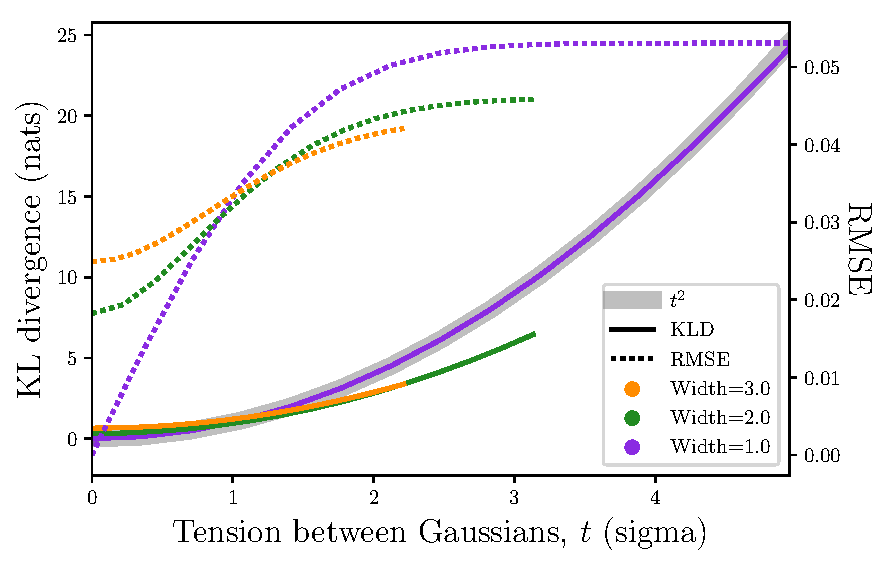
\includegraphics[width=\columnwidth]{figures/tension.pdf}
    \caption{The KLD (solid line) is equal to the square of the tension $t$, 
with a small additive offset when $r\neq1$, whereas the RMSE (dotted line) is 
relatively insensitive to tension past a certain point.
    \label{fig:tension}}
  \end{center}
\end{figure}

\subsection*{Acknowledgments}


The work of PJM was supported by the U.S. Department of Energy under contract 
number DE-AC02-76SF00515.
SJS was partially supported by the National Science Foundation under grant 
N56981CC.


%
%This is the text imported from \code{acknowledgments.tex}, and will be replaced by some standard LSST DESC boilerplate at some point.
%


Author contributions are listed below. \\
A.I.~Malz: Initiated project, led development work. \\
P.J.~Marshall: Advised on statistics, and project design and management. \\
S.J.~Schmidt: Produced the PDFs for the fainter mock catalog. \\
M.L.~Graham: Produced the photometry and PDFs for the brighter mock catalog. \\
J.~DeRose: Produced the photometry for the fainter mock catalog. \\
R.~Wechsler: Supervised production of the fainter mock catalog. \\



\bibliography{lsstdesc,main}

\end{document}
